\chapter{Multiplexer area}
\section{Theoretical analysis}
The area of a single transistor is estimated as the product between the length (L) and the width (W).
The overall length $L$ is the sum of the the gate and the source and drain lengths. For the symmetry of the MOS structure, we can imagine that both source and drain lengths are equal and depend from the gate length according to arbitrary design rules $L_{S/D}= \lambda L_{gate}$. 
\begin{equation}
L = L_{gate} + 2 \ L_{S/D}.
\end{equation}
 The width is different between the two transistors, but the ratio remains always the same ($W_p / W_n =1.29$). In order to evaluate the occupied area of a mux, it is necessary to obtain first the area of a single Nand made with the CMOS technology. Another important aspect to take into account is the interconnections override that has been estimated to be the 15\% of the logic gate area ($I_O=0.15$).
As results, the area of a single Nand2 ($A_{ND2}$) is:
\begin{equation}
A_{ND2}=2L \ (Wn+Wp) (1+I_O)
\end{equation}
Once the occupied area of a single Nand2 is known, it is necessary to know the overall number of gates in the circuit. To do so, we can use the equation \ref{magic} in chapter 2, that allows to do a smart and full estimation of the number of gates in our system.

\section{Simulation results}
Here are reported several tables with the occupation area expressed in $\mu m^2$, for a nMOS with a channel width of 270nm. The program of course allows to make calculations for a customized value of channel width.
\subsubsection{Hp Technology}
\begin{tabular}{|c|c|c|c|c|c|c|}
	\hline
	& \bfseries2x1 & \bfseries8x1 & \bfseries16x1 & \bfseries32x1 & \bfseries64x1 & \bfseries128x1 \\
	\hline
	\hline
	\bfseries8 bit&1.9966&13.9763&29.9492&61.8950&125.7867&253.578\\
	\hline
	\bfseries16 bit&3.9932&27.9526&59.8984&123.7901&251.5734&507.1400 \\
	\hline
	\bfseries32 bit&7.9865&55.9052&119.7569&247.5802&503.1468&1014.3 \\
	\hline
	\bfseries64 bit&15.9729&111.8104&239.5937&495.1604&1006.3& 2028.6 \\
	\hline
\end{tabular} 
\subsubsection{Lop Technology}
\begin{tabular}{|c|c|c|c|c|c|c|}
	\hline
	& \bfseries2x1 & \bfseries8x1 & \bfseries16x1 & \bfseries32x1 & \bfseries64x1 & \bfseries128x1 \\
	\hline
	\hline
	\bfseries8 bit&2.4403&17.0821&36.6046&75.6495&153.7393&309.9189 \\
	\hline
	\bfseries16 bit&4.8806&34.1643&73.2092&151.2990&307.4786&619.8378\\
	\hline
	\bfseries32 bit&9.7612&68.3286&146.4184&302.5980&614.9572&1239.7\\
	\hline
	\bfseries64 bit&19.5225&136.6572&292.8368&605.1960&1229.9&2479.4\\
	\hline
\end{tabular} 
\subsubsection{Lstp Technology}
\begin{tabular}{|c|c|c|c|c|c|c|}
	\hline
	& \bfseries2x1 & \bfseries8x1 & \bfseries16x1 & \bfseries32x1 & \bfseries64x1 & \bfseries128x1 \\
	\hline
	\hline
	\bfseries8 bit&3.1058&21.7409&64.5877&96.2812&195.6682&394.4423 \\
	\hline
	\bfseries16 bit&6.2117&43.4818&93.1753&192.5424&391.3364&788.8845\\
	\hline
	\bfseries32 bit&12.4234&86.9634&186.3507&385.1247&782.6728&1577.8 \\
	\hline
	\bfseries64 bit&24.8468&173.9273&372.7013&770.2495&1565.3&3155.5\\
	\hline
\end{tabular} 

\section{Discussion}
As expected the occupied area shows a net tendency to increase as a function of the parallelism. However, the occupied area of a HP technology is generally smaller than the other technologies.  And the LSTP technology shows the greatest occupied area as a function of number of the parallelism.
\begin{figure}[!]
	\centering
	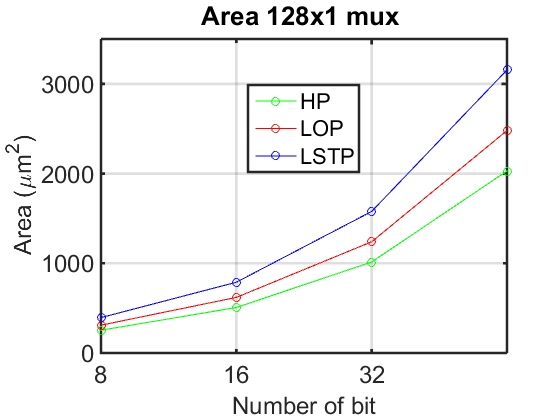
\includegraphics[scale =1]{capitoli/Area128to1}
	\caption{Occupied area of a mux 128x1 as a function of the parallelism}
	\label{fig:area}
	
\end{figure} 
\newpage

\section{Matlab implementation}
In the table below are reported the input data of the main script.

\begin{table}[h]
	\begin{center}
		\begin{tabular}{|c|c|c|c|} \hline
			\textbf{Quantity name} & \textbf{Description} & \textbf{u.m. (S.I.)} & \textbf{Variable name} \\ \hline
			$X$ &Number of input (is a power of 2) & / & X \\ 
			$W$ &Parallelism (is a power of 2) & / & Word \\
			$W_n$ &Gate width & um & Wn \\ 
			$I_O$ &Interconnections override & / &interc\_override \\ 
			$\lambda$ &design parameter to determine $L_{S/D}$ & / & lambda\\
			$L_{gate}$ &Gate length HP, LOP, LSTP 2010 & um & Lgate \\	 \hline
		\end{tabular}
	\end{center}
	\caption{Input data}
	\label{tabn}
\end{table}

In the table below are reported the output data of the main script.

\begin{table}[h]
	\begin{center}
		\begin{tabular}{|c|c|c|c|} \hline
			\textbf{Quantity name} & \textbf{Description} & \textbf{u.m. (S.I.)} & \textbf{Variable name} \\ \hline
			$A_{MUX} \ HP2010$ &Area MUX HP 2010 & $\mu m^2$ & AreaHP \\
			$A_{MUX} \ LOP2010$ &Area MUX LOP 2010 & $\mu m^2$ & AreaLOP \\
			$A_{MUX} \ LSTP2010$ &Area MUX LSTP 2010 & $\mu m^2$ & AreaLSTP \\  \hline
		\end{tabular}
	\end{center}
	\caption{Output data}
	\label{tabna}
\end{table}

\subsection{Main code}
\lstinputlisting{capitoli/main_area.m}